\chapter{Results and performance}
\label{Chapter5}
\lhead{Chapter 5. \emph{Results and performance}}

\todo{Present the results and discuss any differences between the findings and your initial predictions/hypothesis}

\todo{Interpret your experimental results - do not just present lots of data and expect the reader to understand it.
    Evaluate what you have achieved against the aims and objectives you outlined in the introduction}

\section{Hypothesis}
As mentionned in Section \ref{section:research_obj}, the primary objective was to implement a new algorithm in order to find solutions, focusing on the more realistic instances ($I_1 \ldots I_8$) without imposing time constraints.

Hence, simulations for every instances have been conducted, testing different combinations of parameters in what is called a grid search. Each combination of parameters was run 10 times to ensure the reliability and consistency of the results.
One challenge, is that the computational budget is limited when using Python. Especially for the more complex instance, ($I_7 \ldots I_{14}$) where the time to find a solution for a given set of parameters is more than 20 minutes. It becomes practically impossible to perform for each instance, 10 simulations for every combination of parameters in the grid search. Hence, the size of the grid search for the more complex instances were reduced as shown in Table \ref{table:Grid search}.

\begin{table}[!ht]
    \centering
    \caption{Grid search}
    \resizebox{\textwidth}{!}{ % Resize the table to fit the text width
        \begin{tabular}{||>{\centering\arraybackslash}p{3cm}
            >{\centering\arraybackslash}p{4.5cm}
            >{\centering\arraybackslash}p{3.5cm}
            >{\centering\arraybackslash}p{2cm}||}
            \toprule
                                          & ($I_1 \ldots I_6$)        & ($I_7 \ldots I_8$) & ($I_9 \ldots I_{14}$) \\ [1ex]
            \midrule
            \textit{selection\_policies}  & top\_k, ratio\_k          & top\_k, ratio\_k   & -                     \\
            \textit{simulation\_policies} & random, greedy, tolerance & greedy             & -                     \\
            \textit{selection\_policies}  & UCB, UCB1T                & UCB, UCB1T         & -                     \\
            \textit{c\_p}                 & 0, 1.4, 2.8               & 1.4                & -                     \\
            \textit{N\_children}          & 5, 10, 15                 & 10                 & -                     \\
            \textit{Ratio}                & 0, .3, .5, .8, 1          & .5                 & -                     \\
            \bottomrule
        \end{tabular}
    }
    \label{table:Grid search}
\end{table}

\section{Results analysis}
\subsection{Overview}

After running the various simulations with the search grid parameters defined in Table \ref{table:Grid search}, our results were compared with those of Kiwi and RL (Reinforcement Learning) \cite{reinforcement_learning_yaro} - the only two official publications on this challenge.

\begin{table}[!ht]
    \centering
    \caption{Best results vs State of the art}
    \resizebox{.8\textwidth}{!}{ % Resize the table to fit the text width
        \begin{tabular}{||>{\centering\arraybackslash}p{1.5cm}
            >{\centering\arraybackslash}p{1.5cm}
            >{\centering\arraybackslash}p{1.5cm}
            >{\centering\arraybackslash}p{1.5cm}
            >{\centering\arraybackslash}p{1.5cm}
            >{\centering\arraybackslash}p{1.5cm}
            >{\centering\arraybackslash}p{1.5cm} ||}
            \toprule
            Instance & Kiwi's & RL     & Best known & Best found    & Mean    & Std   \\ [1ex]
            \midrule
            I1       & 1396   & 1396   & 1396       & \textbf{1396} & 1396    & 0     \\
            I2       & 1498   & 1498   & 1498       & \textbf{1498} &         &       \\
            I3       & 7672   & 7672   & 7672       & \textbf{7672} &         &       \\
            I4       & 14024  & 13952  & 13952      & 15101         & 16208.8 & 520.8 \\
            I5       & 698    & 690    & 690        & -             & -       & -     \\
            I6       & 2159   & 2610   & 2159       & -             & -       & -     \\
            I7       & 31681  & 30937  & 30937      & -             &         &       \\
            I8       & 4052   & 4081   & 4052       & \textbf{4037} & -       &       \\
            I9       & 76372  & 75604  & 75604      & -             & -       & -     \\
            I10      & 21667  & 58304  & 21667      & -             & -       & -     \\
            I11      & 44153  & 59361  & 44153      & -             & -       & -     \\
            I12      & 65447  & 86074  & 65447      & -             & -       & -     \\
            I13      & 97859  & 166543 & 97859      & -             & -       & -     \\
            I14      & 118811 & 198787 & 118811     & -             & -       & -     \\ [1ex]
            \bottomrule
        \end{tabular}
    }
    \label{table:Best result vs state of the art}
\end{table}

A solution was found for $I_1, \ldots, I_4$ and $I_7, I_8$. The results shown in table \ref{table:Best result vs state of the art} are the best found costs' solution within the grid search. The results of the simulations for $I_1,\ldots I_4$ are displayed in Section \ref{AppendixC} and the detailed path-solution for these instances can be found in Section \ref{AppendixD}.
\newpage
\subsection{Analysis}
\subsubsection{I1, I2 and I3}
For these three instances, the best known solutions were found and the various simulations were carried out successfully. Therefore, the influence of the parameters on the final solution was investigated. For $I_3$, the analysis focuses on the $C_p$ parameter, the influence of the expansion ratio and finally the study will investigate the overall correlation matrix.

\subsubsection*{Analysis on $C_p$}
\begin{figure}[!ht]
    \centering
    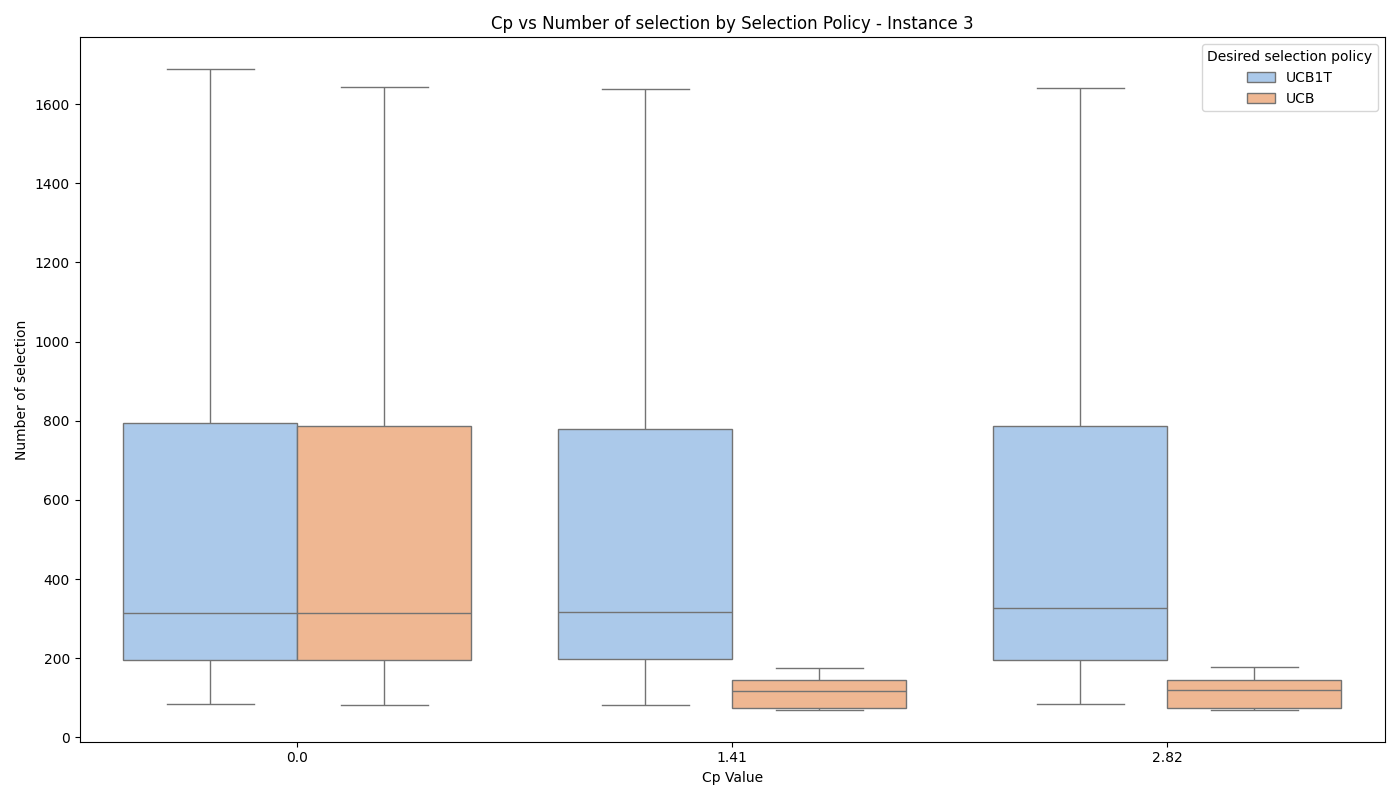
\includegraphics[width=\textwidth]{Figures/3 - cp_vs_selection.png}
    \caption{$C_p$ vs Number of selection}
    \label{fig:cp_vs_selection_3}
\end{figure}

On Figure \ref{fig:cp_vs_cost_3} the box plots illustrate the relationship between the exploration constant \( C_p \) and the number of selection phases under the UCB and UCB1T selection policies:

\begin{itemize}
    \item \textbf{\( C_p = 0 \) lead to the same performance:}
          When the $C_p=0$, the selection policy of the UCB and the UCB1T are the same (cf equation \ref{eq:UCB} and \ref{eq:UCB1T}).
    \item \textbf{Higher \( C_p \) values lead to faster convergence for UCB:}
          As \( C_p \) increases from $0.0$ to $2.82$, the median number of selection phases under UCB policy decreases. A higher number of selection for the UCB policy could be expected, as $C_p$ increases but for small instances it convergences faster.

    \item \textbf{UCB1T Encourages More Exploration:}
          UCB1T consistently results in a higher number of selection phases compared to UCB, especially at higher \( C_p \) values. This is consistent with UCB1T's definition to promote broader exploration before converging.

    \item \textbf{Balance Between Exploration and Exploitation:}
          The choice of \( C_p \) should be based on the specific problem, balancing the need for exploration (higher \( C_p \)) with the desire for quicker convergence (lower \( C_p \)).
\end{itemize}

Although a higher exploration parameter $C_p$ may lead to faster convergence under the UCB selection policy, it often results in worse outcomes compared to the UCB1T algorithm, as shown on Figure \ref{fig:cp_vs_cost_3}.
\begin{figure}[!ht]
    \centering
    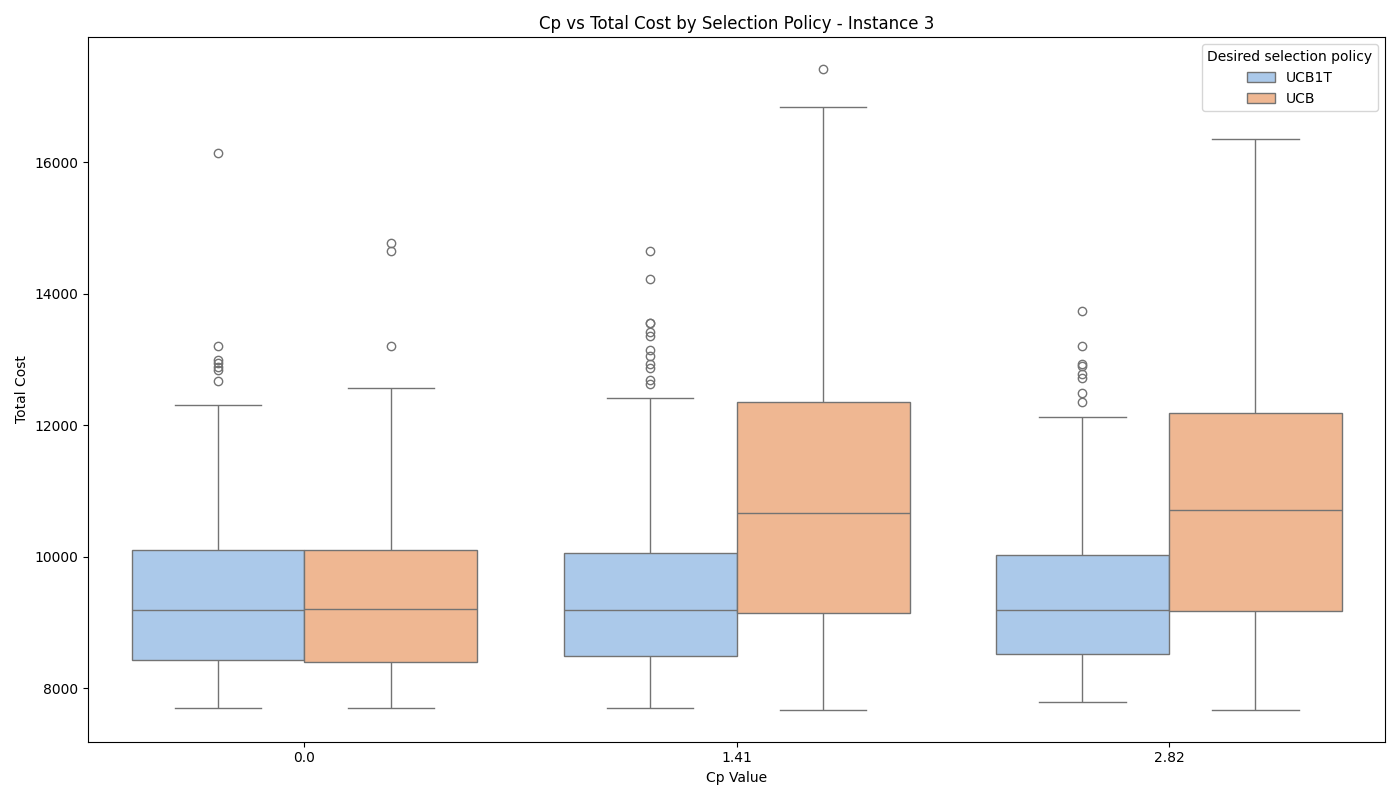
\includegraphics[width=\textwidth]{Figures/3 - cp_vs_cost.png}
    \caption{$C_p$ vs Total cost}
    \label{fig:cp_vs_cost_3}
\end{figure}
While UCB1T may require more time to converge, it generally explores the search tree more effectively, leading to better overall performance.





\subsubsection*{Analysis of Expansion ratio}

\begin{figure}[!ht]
    \centering
    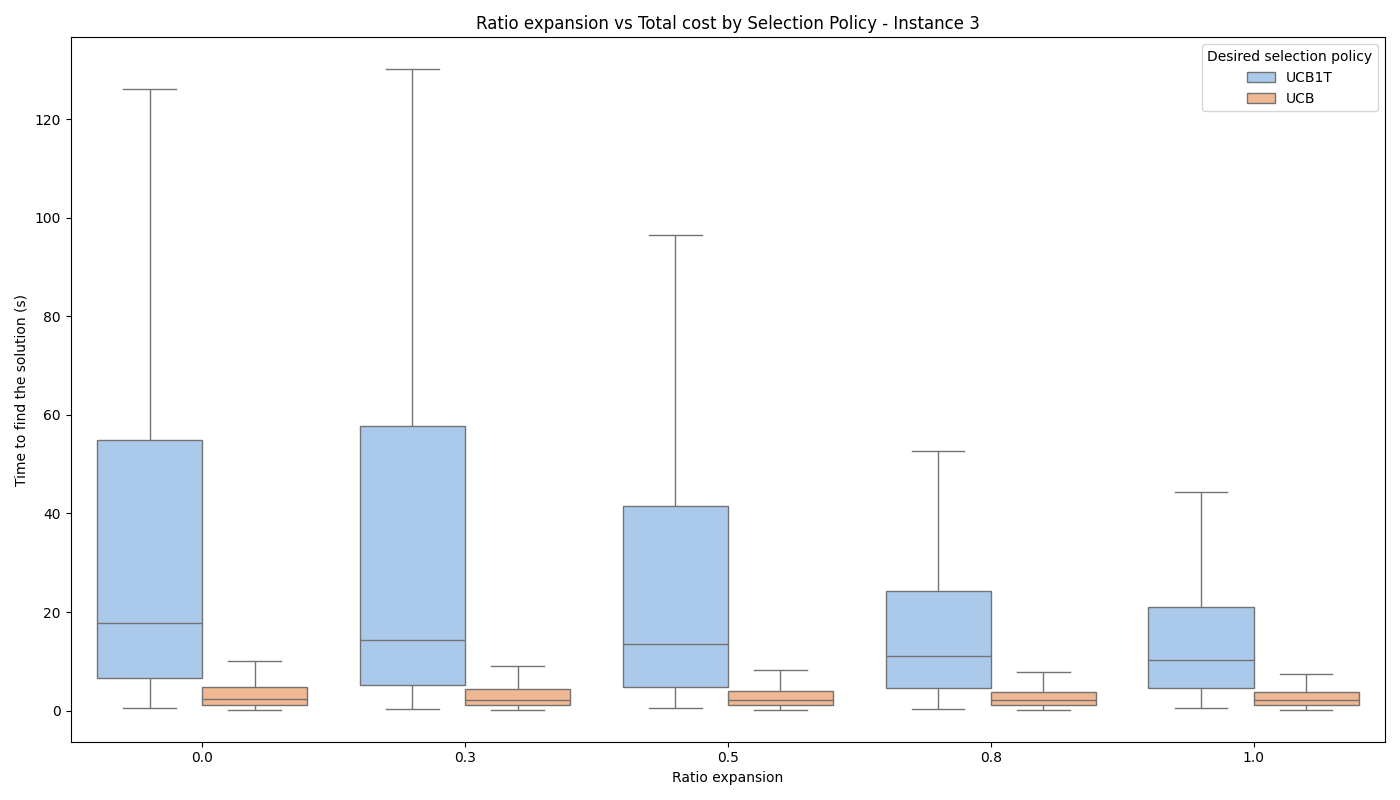
\includegraphics[width=\textwidth]{Figures/3 - ratio_vs_time.png}
    \caption{Ratio expansion vs Time to find the solution}
    \label{fig:Ratio vs Time}
\end{figure}

The box plots show the relationship between ratio expansion (the proportion of expanded child nodes that has the cheapest flight connection over the chosen number of children) and the time to find a solution for the UCB and UCB1T policies:

\begin{itemize}
    \item \textbf{UCB is More Time-Efficient:}
          Across all ratio expansion values, the UCB policy consistently finds solutions more quickly than UCB1T. This suggests that UCB, being less aggressive in exploration, converges on solutions faster.

          %\item \textbf{UCB1T Takes Longer Due to Extensive Exploration:}
          %      UCB1T shows higher and more variable times to find solutions, especially at lower ratio expansions (e.g., $0.0$). This reflects UCB1T's property to explore more than UCB.

    \item \textbf{Higher Ratio Expansions Lead to Quicker Solutions:}
          For both policies, the time to find a solution generally decreases as the ratio expansion increases, indicating a more efficient search process when more expanded nodes lead to solutions. However, in more complex instances, it is crucial to have a ratio $r \in [0.3,0.7]$ to escape potential leaf node.
\end{itemize}

Finally, the UCB policy is more correlated to the expansion ratio than the UCB1T as shown on Figure \ref{fig:ratio_vs_cost_3}.
\begin{figure}[!ht]
    \centering
    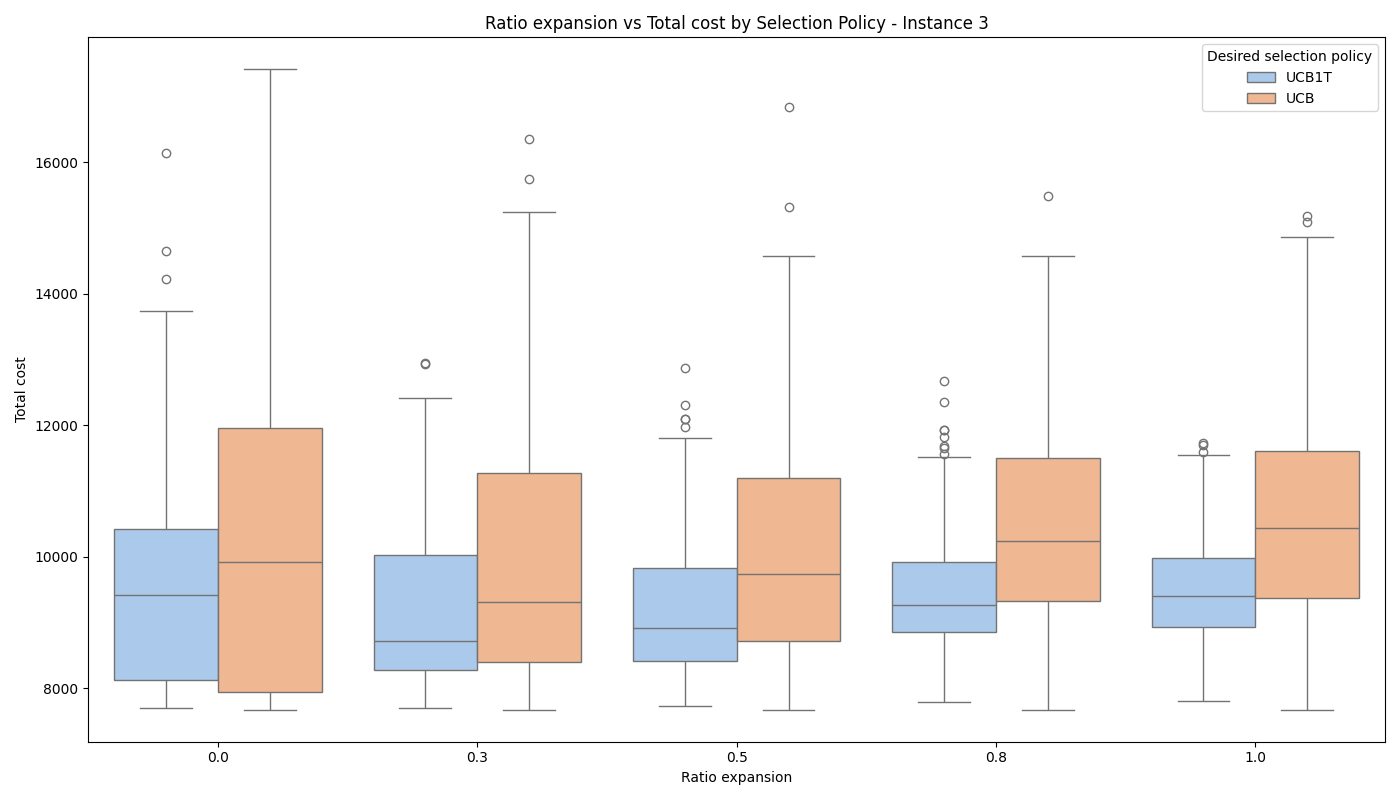
\includegraphics[width=\textwidth]{Figures/3 - ratio_vs_cost.png}
    \caption{Expansion ratio vs Total cost}
    \label{fig:ratio_vs_cost_3}
\end{figure}

UCB's overall performance is worst than UCB1T because it relies heavily on the exploitation compared to UCB1T that even if it converges slower gives better result.


\subsubsection{I5 and I6}

The challenge faced with these two instances is that the defined selection, simulation and expansion policy were not robust enough to explore the tree effectively.

After all the simulations, some nodes in the tree—under the random policy, were able to simulate until reaching a final state. However, due to the randomness of the policy, the tree was pruned at each further iteration where a solution could not be found.

\subsubsection{I4, I7 and I8}

For these instances we have found